% !TEX root = ../report.tex

\section{Logical View}
\label{sec:viewlogical}

% Logical view : The logical view is concerned with the functionality that the system provides to end-users. UML Diagrams used to represent the logical view include Class diagram, Communication diagram, Sequence diagram.

Docker is made using the the go language created by Google. Docker is an application categorized as ``Operating-system-level virtualization''. It consists of:
\begin{itemize}
\item 2979205 lines of go code (almost 3 million).
\item 1782 '.go' files
\item 267 different packages
\end{itemize}

Several tools have been used to get information about the dependencies of the different packages \cite{goviz} \cite{godepgraph}. Using these tools, statistics can be generated about the usage of the packages. This can give an insight about the most important packages of the system.\\
The packages that are most used by other packages is listed below.

\begin{tabular}{l l l}
\textbf{In} & \textbf{Out} & \textbf{Package} \\
%23 & 10 & github.com/docker/notary/tuf/data \\
%24 & 1 & github.com/docker/docker/pkg/stringid \\
%25 & 0 & golang.org/x/net/context \\
%25 & 2 & github.com/docker/docker/pkg/idtools \\
%26 & 2 & github.com/docker/docker/pkg/ioutils \\
%27 & 20 & github.com/docker/docker/layer \\
%29 & 1 & github.com/docker/docker/pkg/system \\
33 & 11 & github.com/docker/docker/image \\
33 & 23 & github.com/docker/docker/pkg/archive \\
36 & 0 & github.com/docker/distribution/digest \\
37 & 5 & github.com/docker/docker/reference \\
37 & 12 & github.com/docker/docker/daemon/execdriver \\
40 & 47 & github.com/docker/docker/container \\
42 & 0 & github.com/opencontainers/runc/libcontainer/configs \\
42 & 4 & github.com/docker/docker/errors \\
43 & 0 & github.com/docker/libnetwork/types \\
47 & 20 & github.com/docker/docker/runconfig \\
48 & 4 & github.com/docker/docker/cli \\
55 & 1 & github.com/docker/docker/pkg/mflag \\
104 & 9 & github.com/docker/docker/api/types \\
187 & 0 & github.com/Sirupsen/logrus \\
\end{tabular} 

The most referenced package is the logging package called ``logrus''. After that it is the api package that is most referenced. This is to be expected, since it is the only way to communicate with the docker daemon \cite{dockerapi}. \\
The ``pkg'' package, the third most referenced package, is, ``a collection of utility packages used by the Docker project without being specific to its internals.''. This means that it can contain any kind of logic for which the developers decided that it should not go in to the core codebase in order to keep the core small \cite{dockerpkg}. The specific mkflag package that is referenced here, is responsible for parsing the multiple flags (hence mflag) that are passed to the command-line interface \cite{dockermflag}. \\
The command line interface (cli) package is most used after this. The docker container package seems to be used by a lot of packages (In) and reference a lot of packages itself as well (Out). Same goes for the docker daemon and the docker image with increasingly less references. \\
Next, the the packages that have the most references to other packages are listed.

\begin{tabular}{l l l}
%2 & 35 & github.com/docker/docker/daemon/execdriver/native \\
1 & 36 & github.com/docker/docker/builder/dockerfile \\
19 & 38 & github.com/docker/docker/registry \\
10 & 43 & github.com/opencontainers/runc/libcontainer \\
0 & 43 & github.com/docker/docker/docker \\
9 & 44 & github.com/docker/docker/api/client/lib \\
40 & 47 & github.com/docker/docker/container \\
10 & 68 & github.com/docker/libnetwork \\
1 & 101 & github.com/docker/docker/distribution \\
1 & 235 & github.com/docker/docker/api/client \\
11 & 349 & github.com/docker/docker/daemon \\
\end{tabular}

Not surprisingly, the docker daemon has the most references. This is because it is responsible for making the containers run in a secure and reliable way. While at the same time the daemon handles requests coming from the API, which is the package with the second most amount of outgoing references.\\
The container package has a lot of references to the runc package, which is a ``CLI tool for spawning and running containers according to the Open Container Format (OCF) specification.'' \cite{opencontainersrunc}. \\

If the main ``/docker'' package is build, containing the functionality of docker, the dependencies can be visualized using a visualization tool. This generates an image that closely resembles the image found in the official documentation \ref{fig:dockerarchipic}.

\begin{figure}[H]
\captionsource{A high-level overview of the Docker architecture}{\cite{dockerarchi}}
\centering
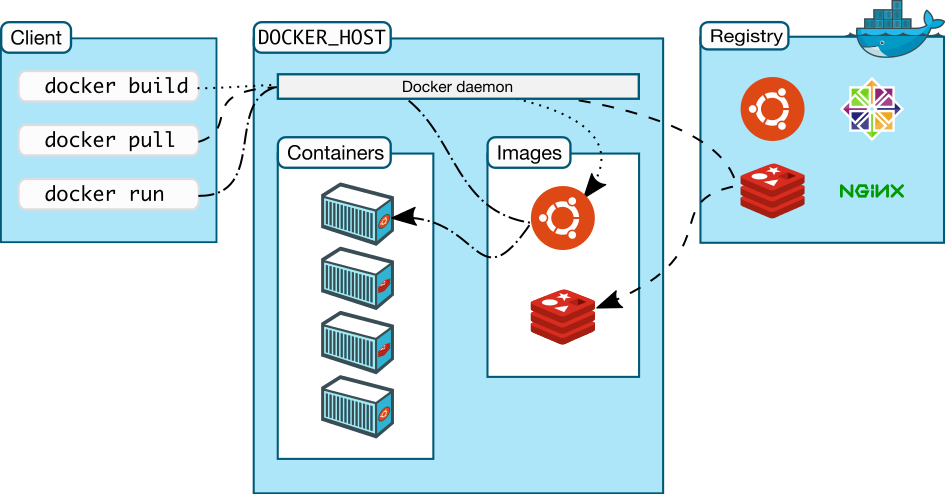
\includegraphics[scale=0.4]{4-softwarearch/images/architecture.png}
\label{fig:dockerarchipic}
\end{figure}
Docker uses a client-server architecture. The client (a command-line tool) acts as the primary user interface and talks to the Docker daemon. The daemon is a background process which does all the heavy lifting, e.g. the building and running of the containers.

The following sections will discuss the most important parts of docker in more detail.

\subsection{Client}
The client is a small binary and acts as the primary user interface to Docker. The user inputs commands into the client and the client forwards these commands to the Docker daemon, which executes commands.
The Docker client is capable of connecting to daemons running on the local machine, as well as connecting to daemons running on remote machines over the internet.

\subsection{Server / Daemon}
The Docker daemon is a process running on the host machine (as can be seen in Figure~\ref{fig:dockerarchipic}). This process is usually started when the host machine starts and runs in the background. It exposes a REST interface and listens for requests coming from clients on the same or remote hosts.

\subsubsection{Images}
Docker images can be interpreted as a read-only template from which Docker containers are
started. A Docker image consists of a stack of layers which are bonded by a union file system. These layers support reusability and sharing.

Docker images can be built from text files (`Dockerfiles'), which contain instructions like installing software and copying files.

\subsubsection{Containers}
% running usin libcontainer from the open specification
Docker containers are based on Docker images. These images consist of read-only
layers. Docker containers contain an additional thin writable layer on top of the images to
perform operations on them. Docker containers basically consist of the files of the operating system,
user-added files, application files, and data files. Multiple containers may run
based on the same image. In this case, Docker will not create separate copies for
each containers. Instead, they will share the same image with their own writable layer.

To run Docker containers, Docker uses the \verb|libcontainer| library, which is part of the Open Container Initiative.

\subsection{Registry}
A Docker registry is a place where Docker images can be stored and retrieved. The Docker daemon
fetches desired Docker images from this repository. This registry can be either public or private and may thus reside behind a firewall. Docker
Hub\footnote{\url{https://hub.docker.com/}} is one example of a docker registry
hosted by Docker. A registry provides an easy way to distribute images among different hosts.
